% Figura cuerpo B1: la curva de Phillips leída como menú de política económica (Samuelson-Solow)
\documentclass[tikz,border=3pt]{standalone}
\usepackage[T1]{fontenc}
\usepackage[utf8]{inputenc}
\usetikzlibrary{arrows.meta,calc,positioning}
\begin{document}
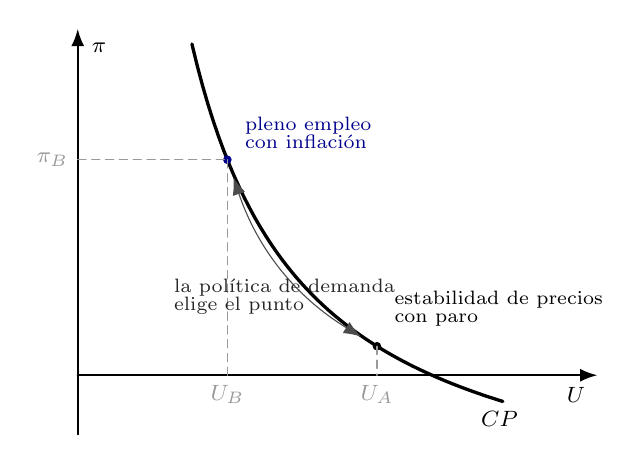
\begin{tikzpicture}[>={Latex[length=2.2mm]}, line cap=round, font=\footnotesize,
  eje/.style={->, thick},
  curva/.style={very thick},
  guia/.style={densely dashed, gray!80},
  pto/.style={circle, fill=black, inner sep=1.1pt}]
  \draw[eje] (0,-0.75) -- (0,4.4) node[below right=2pt]{$\pi$};
  \draw[eje] (0,0) -- (6.6,0) node[below left=1pt]{$U$};
  \draw[curva, domain=1.45:5.4, samples=60] plot (\x,{9*(1/\x-0.22222)});
  \node[anchor=west] at (5.0,-0.55) {$CP$};
  \node[pto, fill=blue!55!black] (B) at (1.9,2.737) {};
  \node[anchor=south west, blue!55!black, align=left] at (2.0,2.75) {\scriptsize pleno empleo\\[-3pt]\scriptsize con inflación};
  \node[pto] (A) at (3.8,0.368) {};
  \node[anchor=south west, align=left] at (3.9,0.5) {\scriptsize estabilidad de precios\\[-3pt]\scriptsize con paro};
  \draw[guia] (1.9,2.737) -- (1.9,0) node[below]{$U_B$};
  \draw[guia] (0,2.737) node[left]{$\pi_B$} -- (1.9,2.737);
  \draw[guia] (3.8,0.368) -- (3.8,0) node[below]{$U_A$};
  \draw[<->, gray!60!black, shorten >=5pt, shorten <=5pt] (A) to[bend left=20] (B);
  \node[gray!30!black, align=left, anchor=west] at (1.1,1.0) {\scriptsize la política de demanda\\[-3pt]\scriptsize elige el punto};
\end{tikzpicture}
\end{document}
